% !TeX root = ../../Skript.tex
\cohead{\Large\textbf{Lineare Funktionen - Einführung}}
\fakesubsection{Einführung}

Alle Funktionen vom Typ \(f(x)=mx+b\) werden als lineare Funktionen bezeichnet.
\begin{tcolorbox}
	\centering\textcolor{loestc}{m: Steigung \qquad	b: y-Achsenabschnitt}
\end{tcolorbox}

Beispiel: \(f(x)=\frac{1}{2}x+1\)

\adjustbox{valign=t, padding = 0ex 0ex 0ex 0ex}{\begin{minipage}{\textwidth}%
    \iftoggle{qrcode}{%
        \settototalheight{\imgheight}{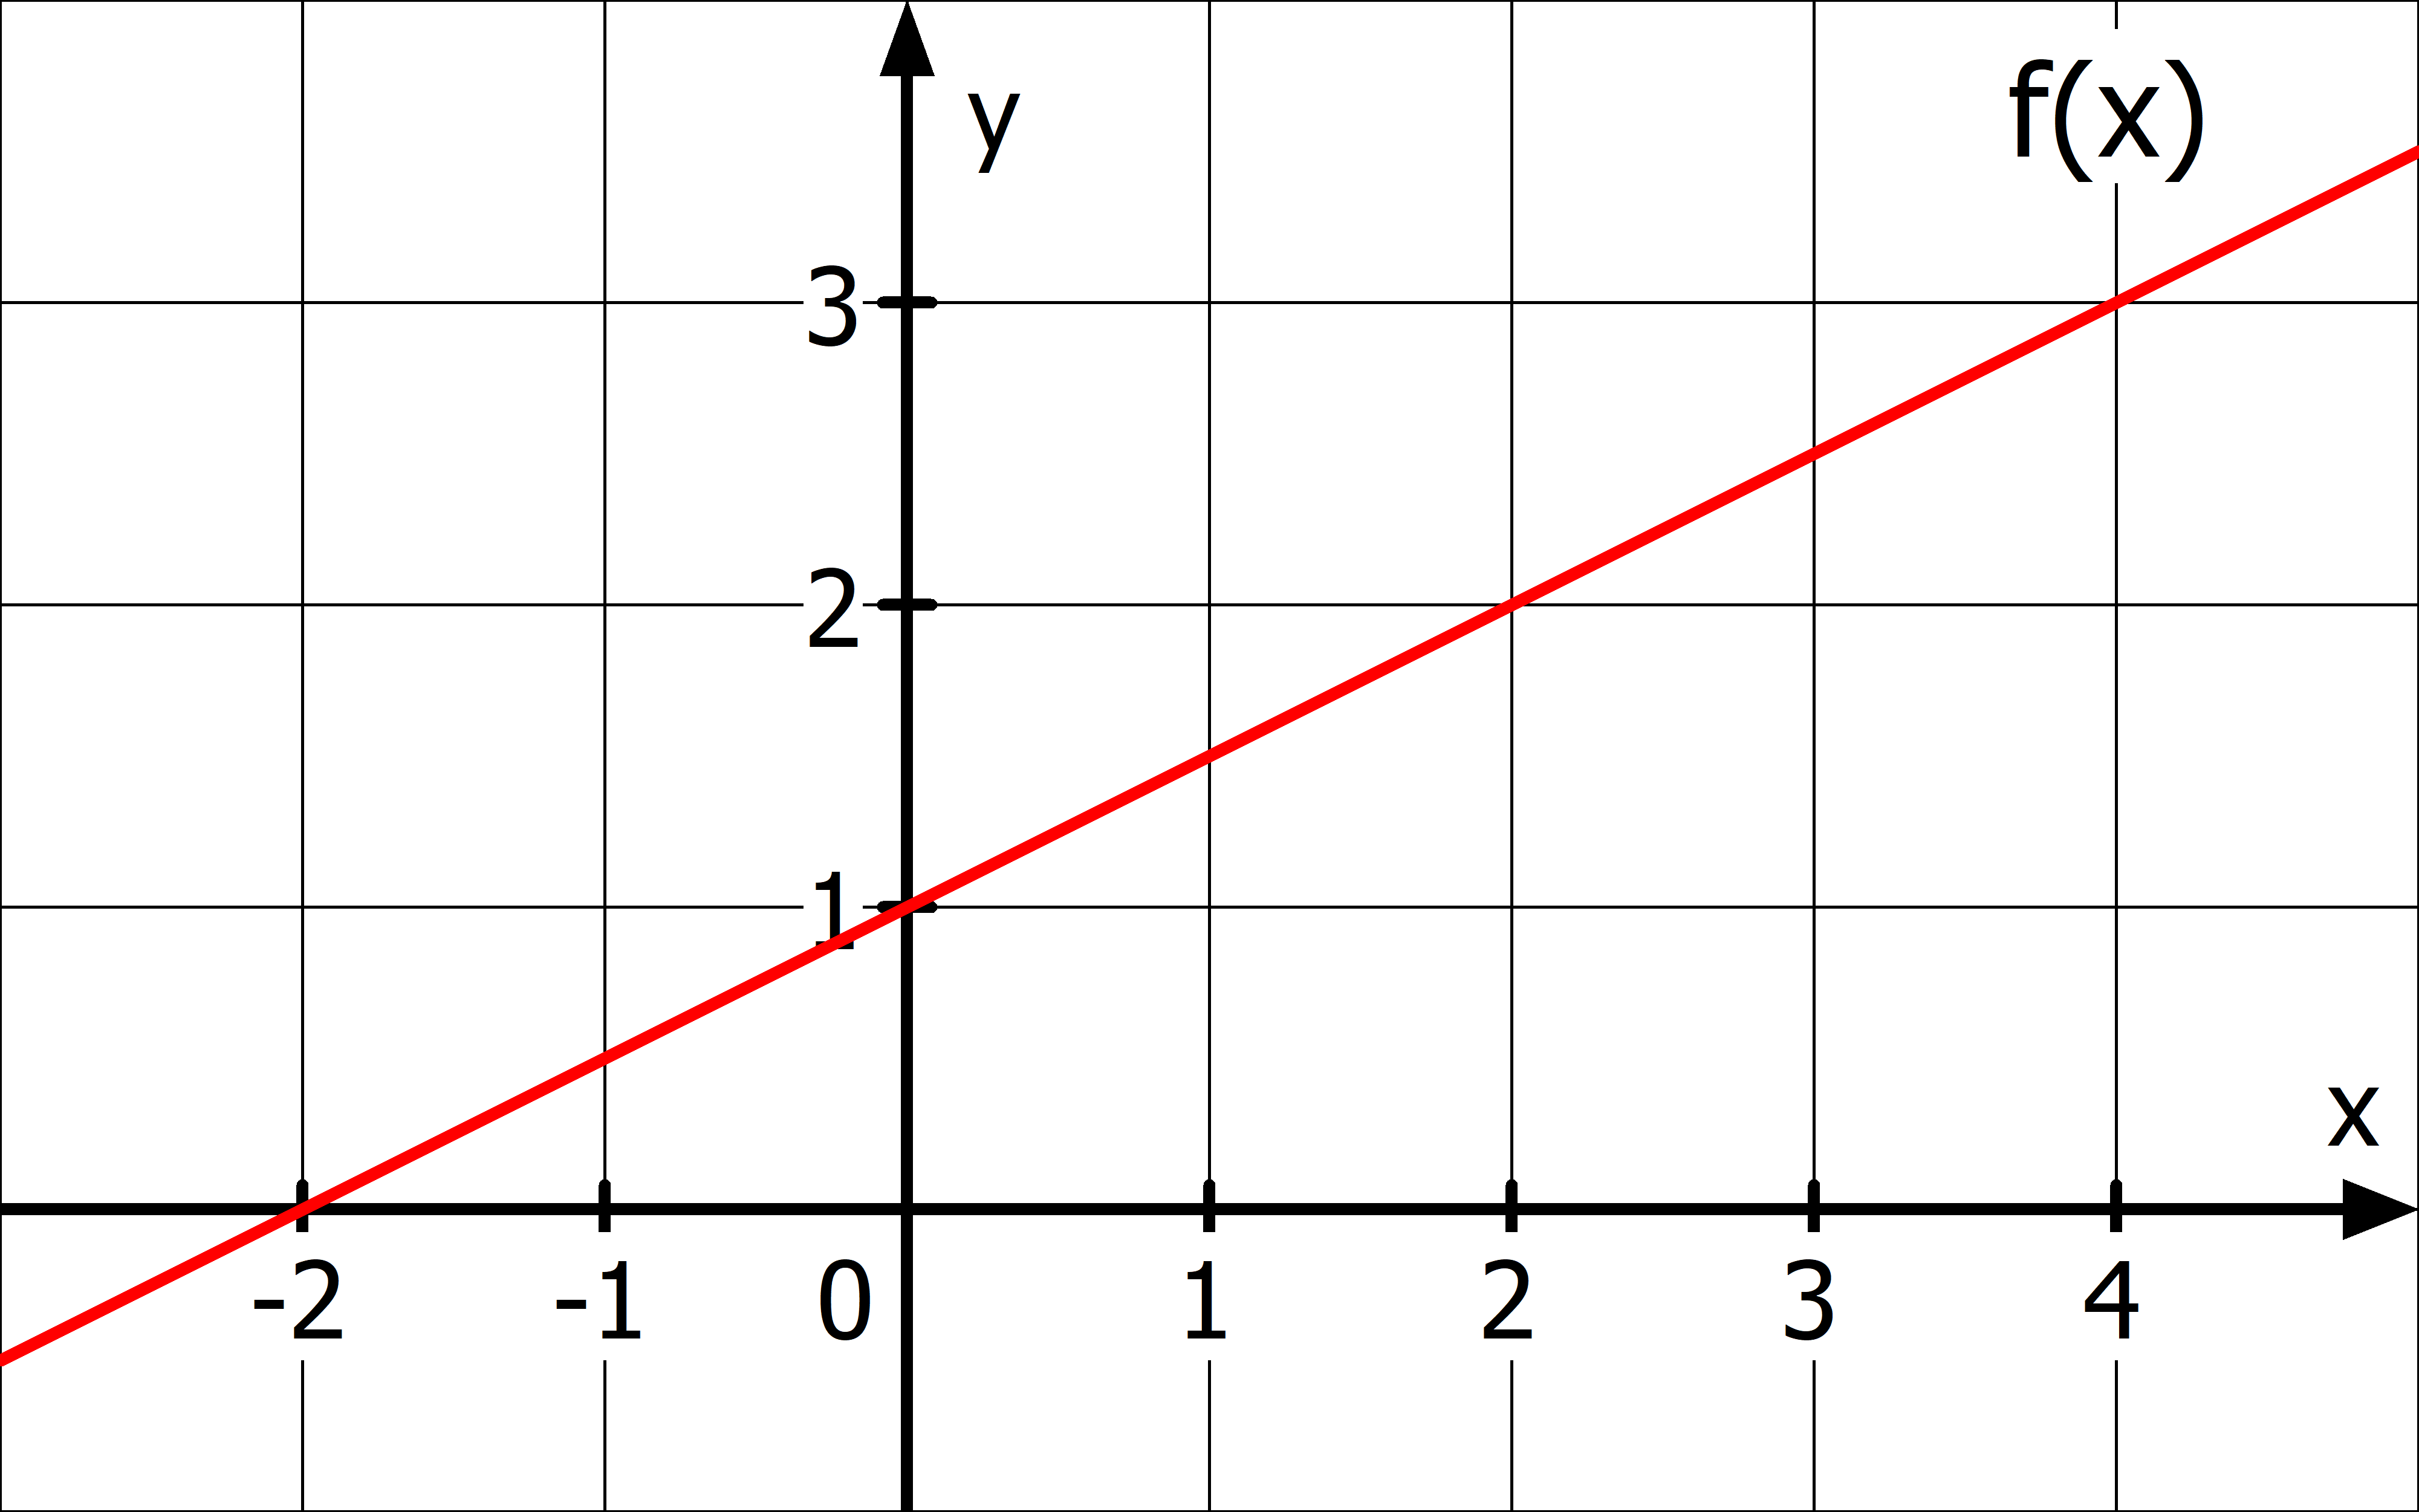
\includegraphics[width=\linewidth]{\linFkt/pics/einfuehrung.png}}%
        \setlength{\qrheight}{2.5cm}%
        \includegraphics[width=\linewidth]{\linFkt/pics/einfuehrung\AUSGEFUELLT.png}%
        \adjustbox{raise=\imgheight-\qrheight, lap=-\textwidth}{\makebox[0pt][l]{\href{https://www.geogebra.org/m/gsantmrf}{
\includegraphics[height=\qrheight]{\linFkt/pics/einfuehrungQR.png}}}}
    }{%
        \includegraphics[width=\linewidth]{\linFkt/pics/einfuehrung\AUSGEFUELLT.png}
    }%
\end{minipage}}%

\medskip

Der y-Achsenabschnitt kann an der y-Achse bei \(x=0\) abgelesen werden. Der y-Achsenabschnitt kann auch immer berechnet werden, indem man \(x=0\) in die Funktion einsetzt:
\begin{align*}
    f(\textcolor{red}{0})=\textcolor{loes}{\frac{1}{2}\cdot 0+1=0+1=1}
\end{align*}

Das Schaubild der Funktion schneidet die y-Achse also bei \(y=\textcolor{loes}{1}\)\textcolor{loes}{.}

Die Steigung kann über das Steigungsdreieck bestimmt werden. Man bestimmt zwei Punkte \(P_1(x_1|y_1)\) und \(P_2(x_2|y_2)\), durch die das Schaubild verläuft und bestimmt dann das Verhältnis des Unterschieds der y-Werte zum Unterschied der x-Werte:
\begin{tcolorbox}
	\centering\textcolor{loestc}{\(m=\dfrac{y_2-y_1}{x_2-x_1}=\dfrac{y_1-y_2}{x_1-x_2}=\dfrac{\Delta y}{\Delta x}\)}
\end{tcolorbox}
Die beiden Punkte können beliebig gewählt werden (sie dürfen nur nicht identisch sein), d.h. das Steigungsdreieck kann an beliebiger Stelle und beliebig groß gezeichnet werden.

Im Beispiel kann man die beiden Punkte \(P_1(\textcolor{red}{-2}|\textcolor{red}{0})\) und \(P_2(\textcolor{blue}{4}|\textcolor{blue}{3})\) wählen oder auch \(P_3(\textcolor{ForestGreen}{0}|\textcolor{ForestGreen}{1})\) und \(P_4(\textcolor{YellowOrange}{2}|\textcolor{YellowOrange}{2})\):
\begin{align*}
	\textcolor{loes}{m=\frac{3-0}{4-(-2)}=\frac{3}{6}=\frac{1}{2}
	\qquad
	m=\frac{2-1}{2-0}=\frac{1}{2}}
\end{align*}

\medskip

Die beiden Geraden \(f(x)=x\) und \(g(x)=-x\) nennt man die erste und zweite Winkelhalbierende, da sie jeweils den \(90^\circ\)-Winkel zwischen der \(x\)- und \(y\)-Achse halbieren.
\newpage
\begin{Exercise}[title={Zeichne das Schaubild der folgenden Funktionen}, label=lineareFktEinfuehrungA1]

	Nutze das ganze Koordinatensystem aus.

	\begin{minipage}[t]{\textwidth}
		\begin{tabular}{cc}
			\centering
			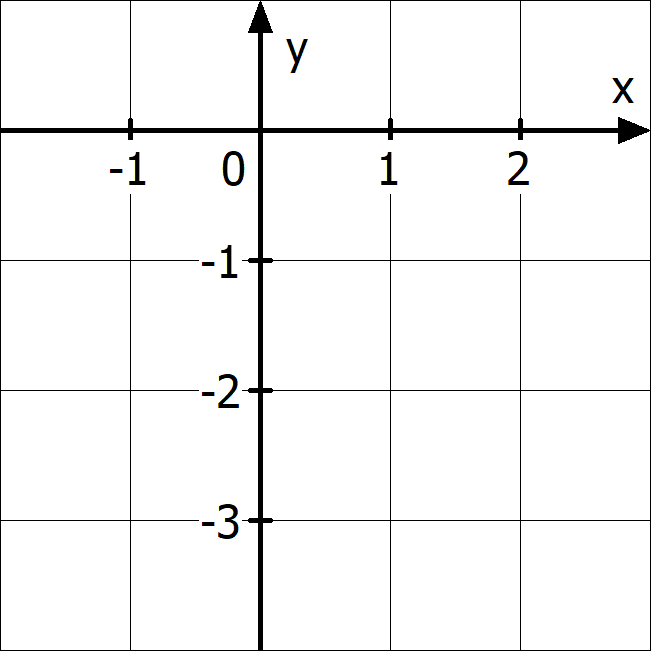
\includegraphics[width=0.4\textwidth]{\linFkt/pics/einfuehrungA1.png}&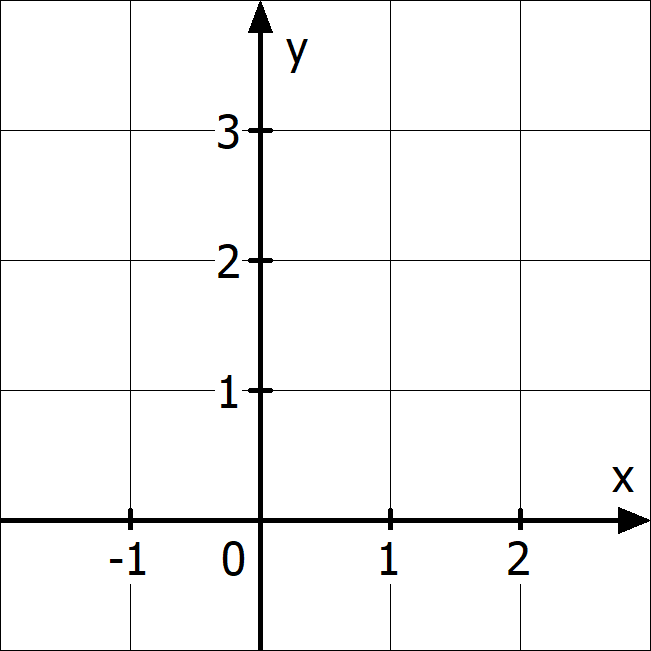
\includegraphics[width=0.4\textwidth]{\linFkt/pics/einfuehrungA2.png}\\
			\(f_1(x)=2x-3\)&	\(f_2(x)=-x+2\)\\ \addlinespace[20pt]
			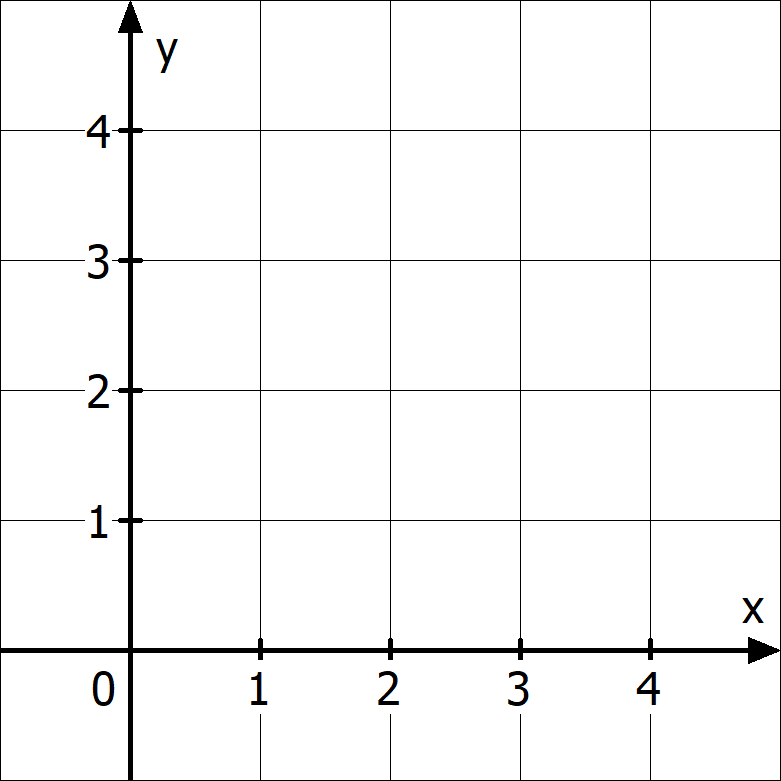
\includegraphics[width=0.4\textwidth]{\linFkt/pics/einfuehrungA3.png}&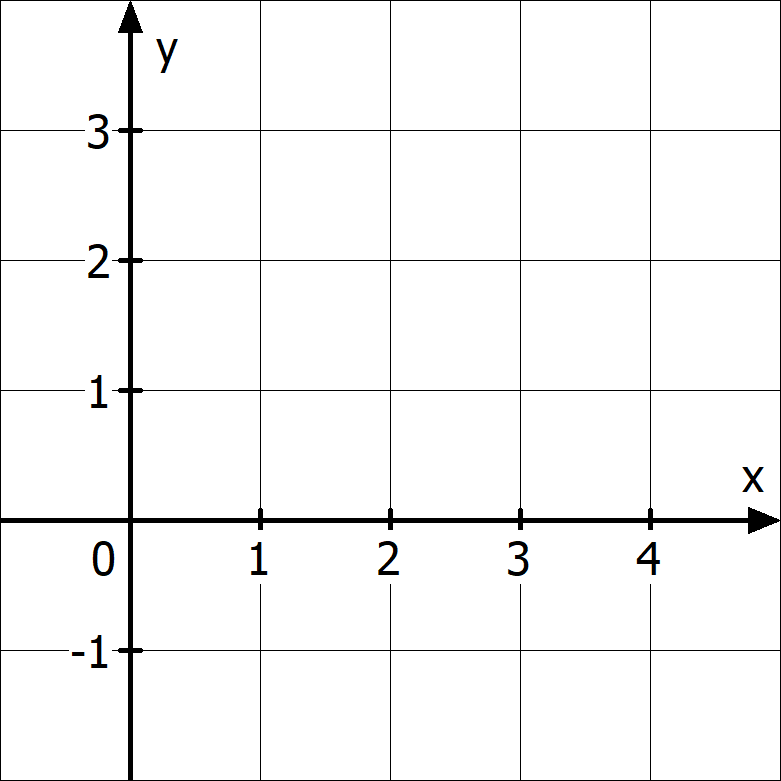
\includegraphics[width=0.4\textwidth]{\linFkt/pics/einfuehrungA4.png}\\
			\(f_3(x)=\frac{3}{4}x+1\)&	\(f_4(x)=-\frac{4}{3}x+3\)
		\end{tabular}
\end{minipage}
\end{Exercise}
\newpage
\begin{Exercise}[title={Bestimme die Funktionsgleichung}, label=lineareFktEinfuehrungA2]\\
	\begin{minipage}[t]{\textwidth}
		\begin{tabular}{cc}
			\centering
			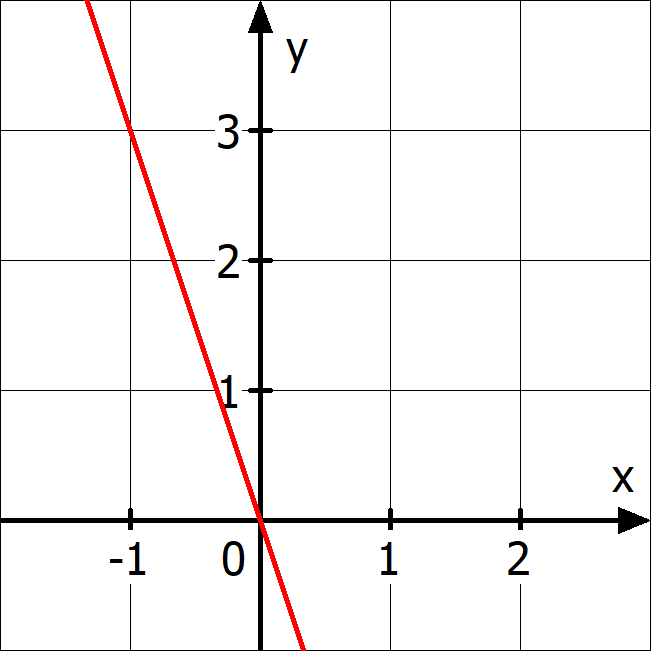
\includegraphics[width=0.4\textwidth]{\linFkt/pics/einfuehrungA5.png}&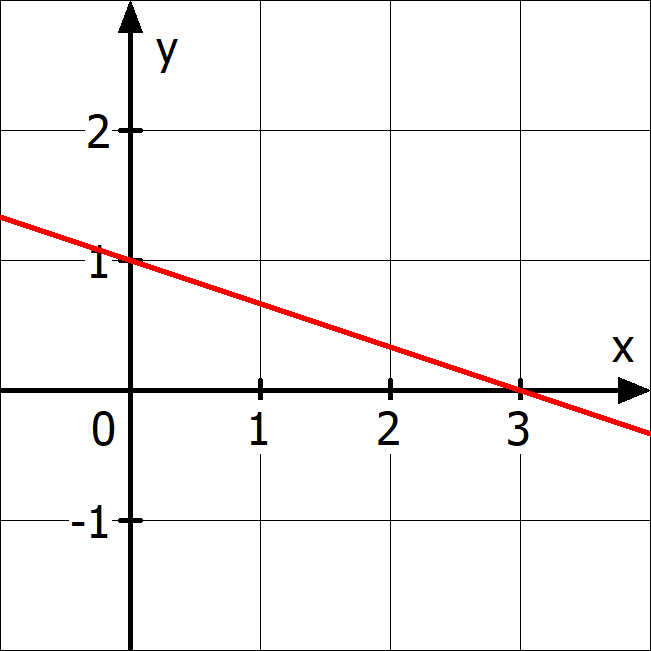
\includegraphics[width=0.4\textwidth]{\linFkt/pics/einfuehrungA6.png}  \\
			\(f_5(x)=\qquad\qquad\qquad\qquad\qquad\)&	\(f_6(x)=\qquad\qquad\qquad\qquad\qquad\)  \\ \addlinespace[20pt]
			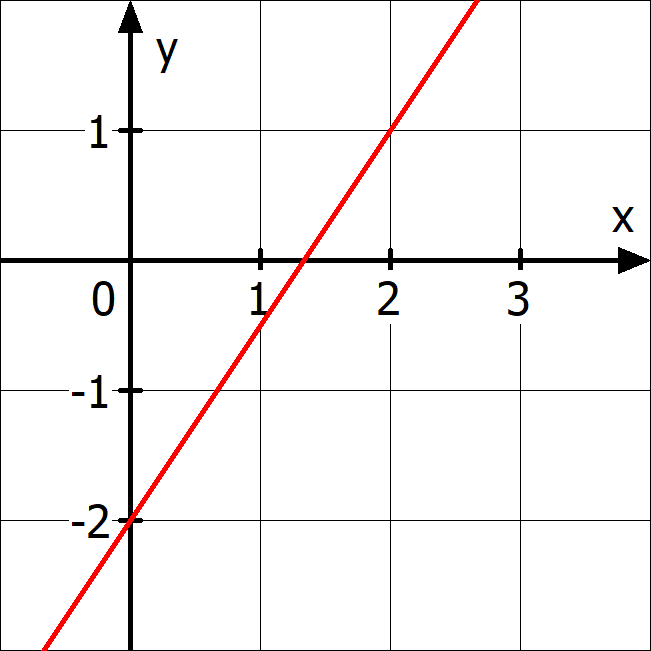
\includegraphics[width=0.4\textwidth]{\linFkt/pics/einfuehrungA7.png}&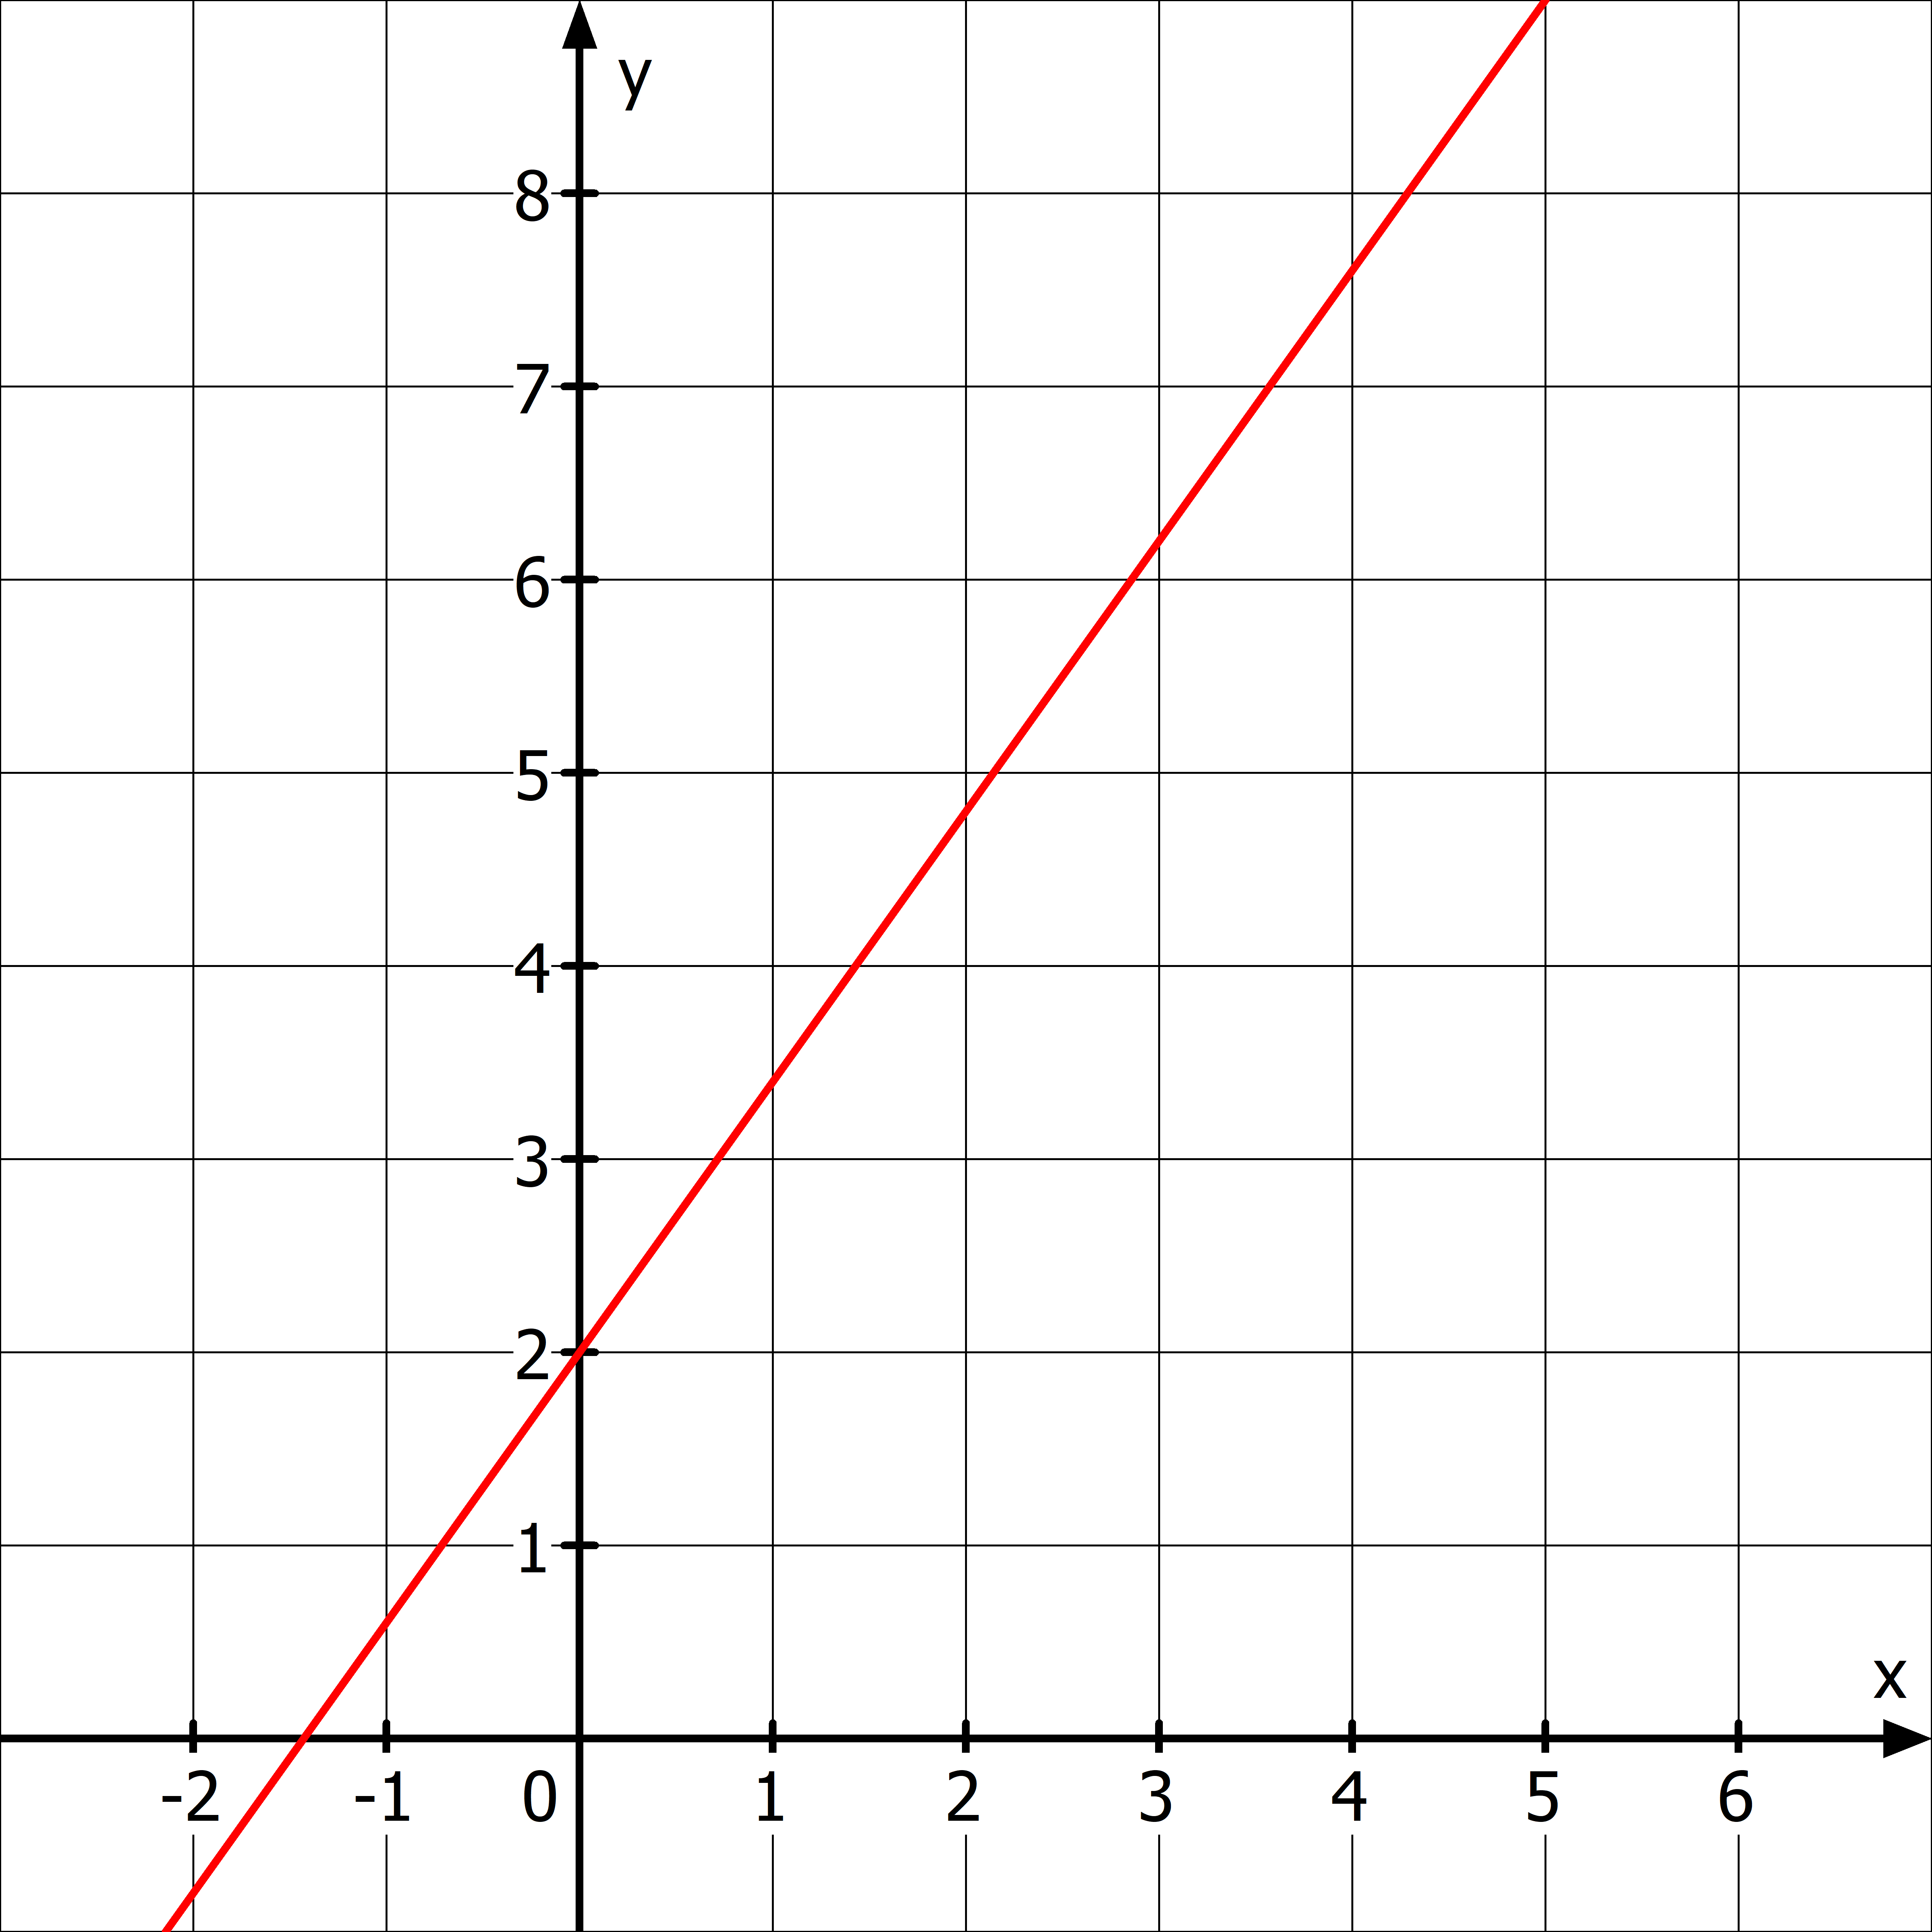
\includegraphics[width=0.4\textwidth]{\linFkt/pics/einfuehrungA8.png}  \\
			\(f_7(x)=\qquad\qquad\qquad\qquad\qquad\)&	\(f_8(x)=\qquad\qquad\qquad\qquad\qquad\)  \\
		\end{tabular}
\end{minipage}
\end{Exercise}
\newpage
\begin{Answer}[ref=lineareFktEinfuehrungA1]

	\begin{minipage}[t]{\textwidth}
		\begin{tabular}{cc}
			\centering
			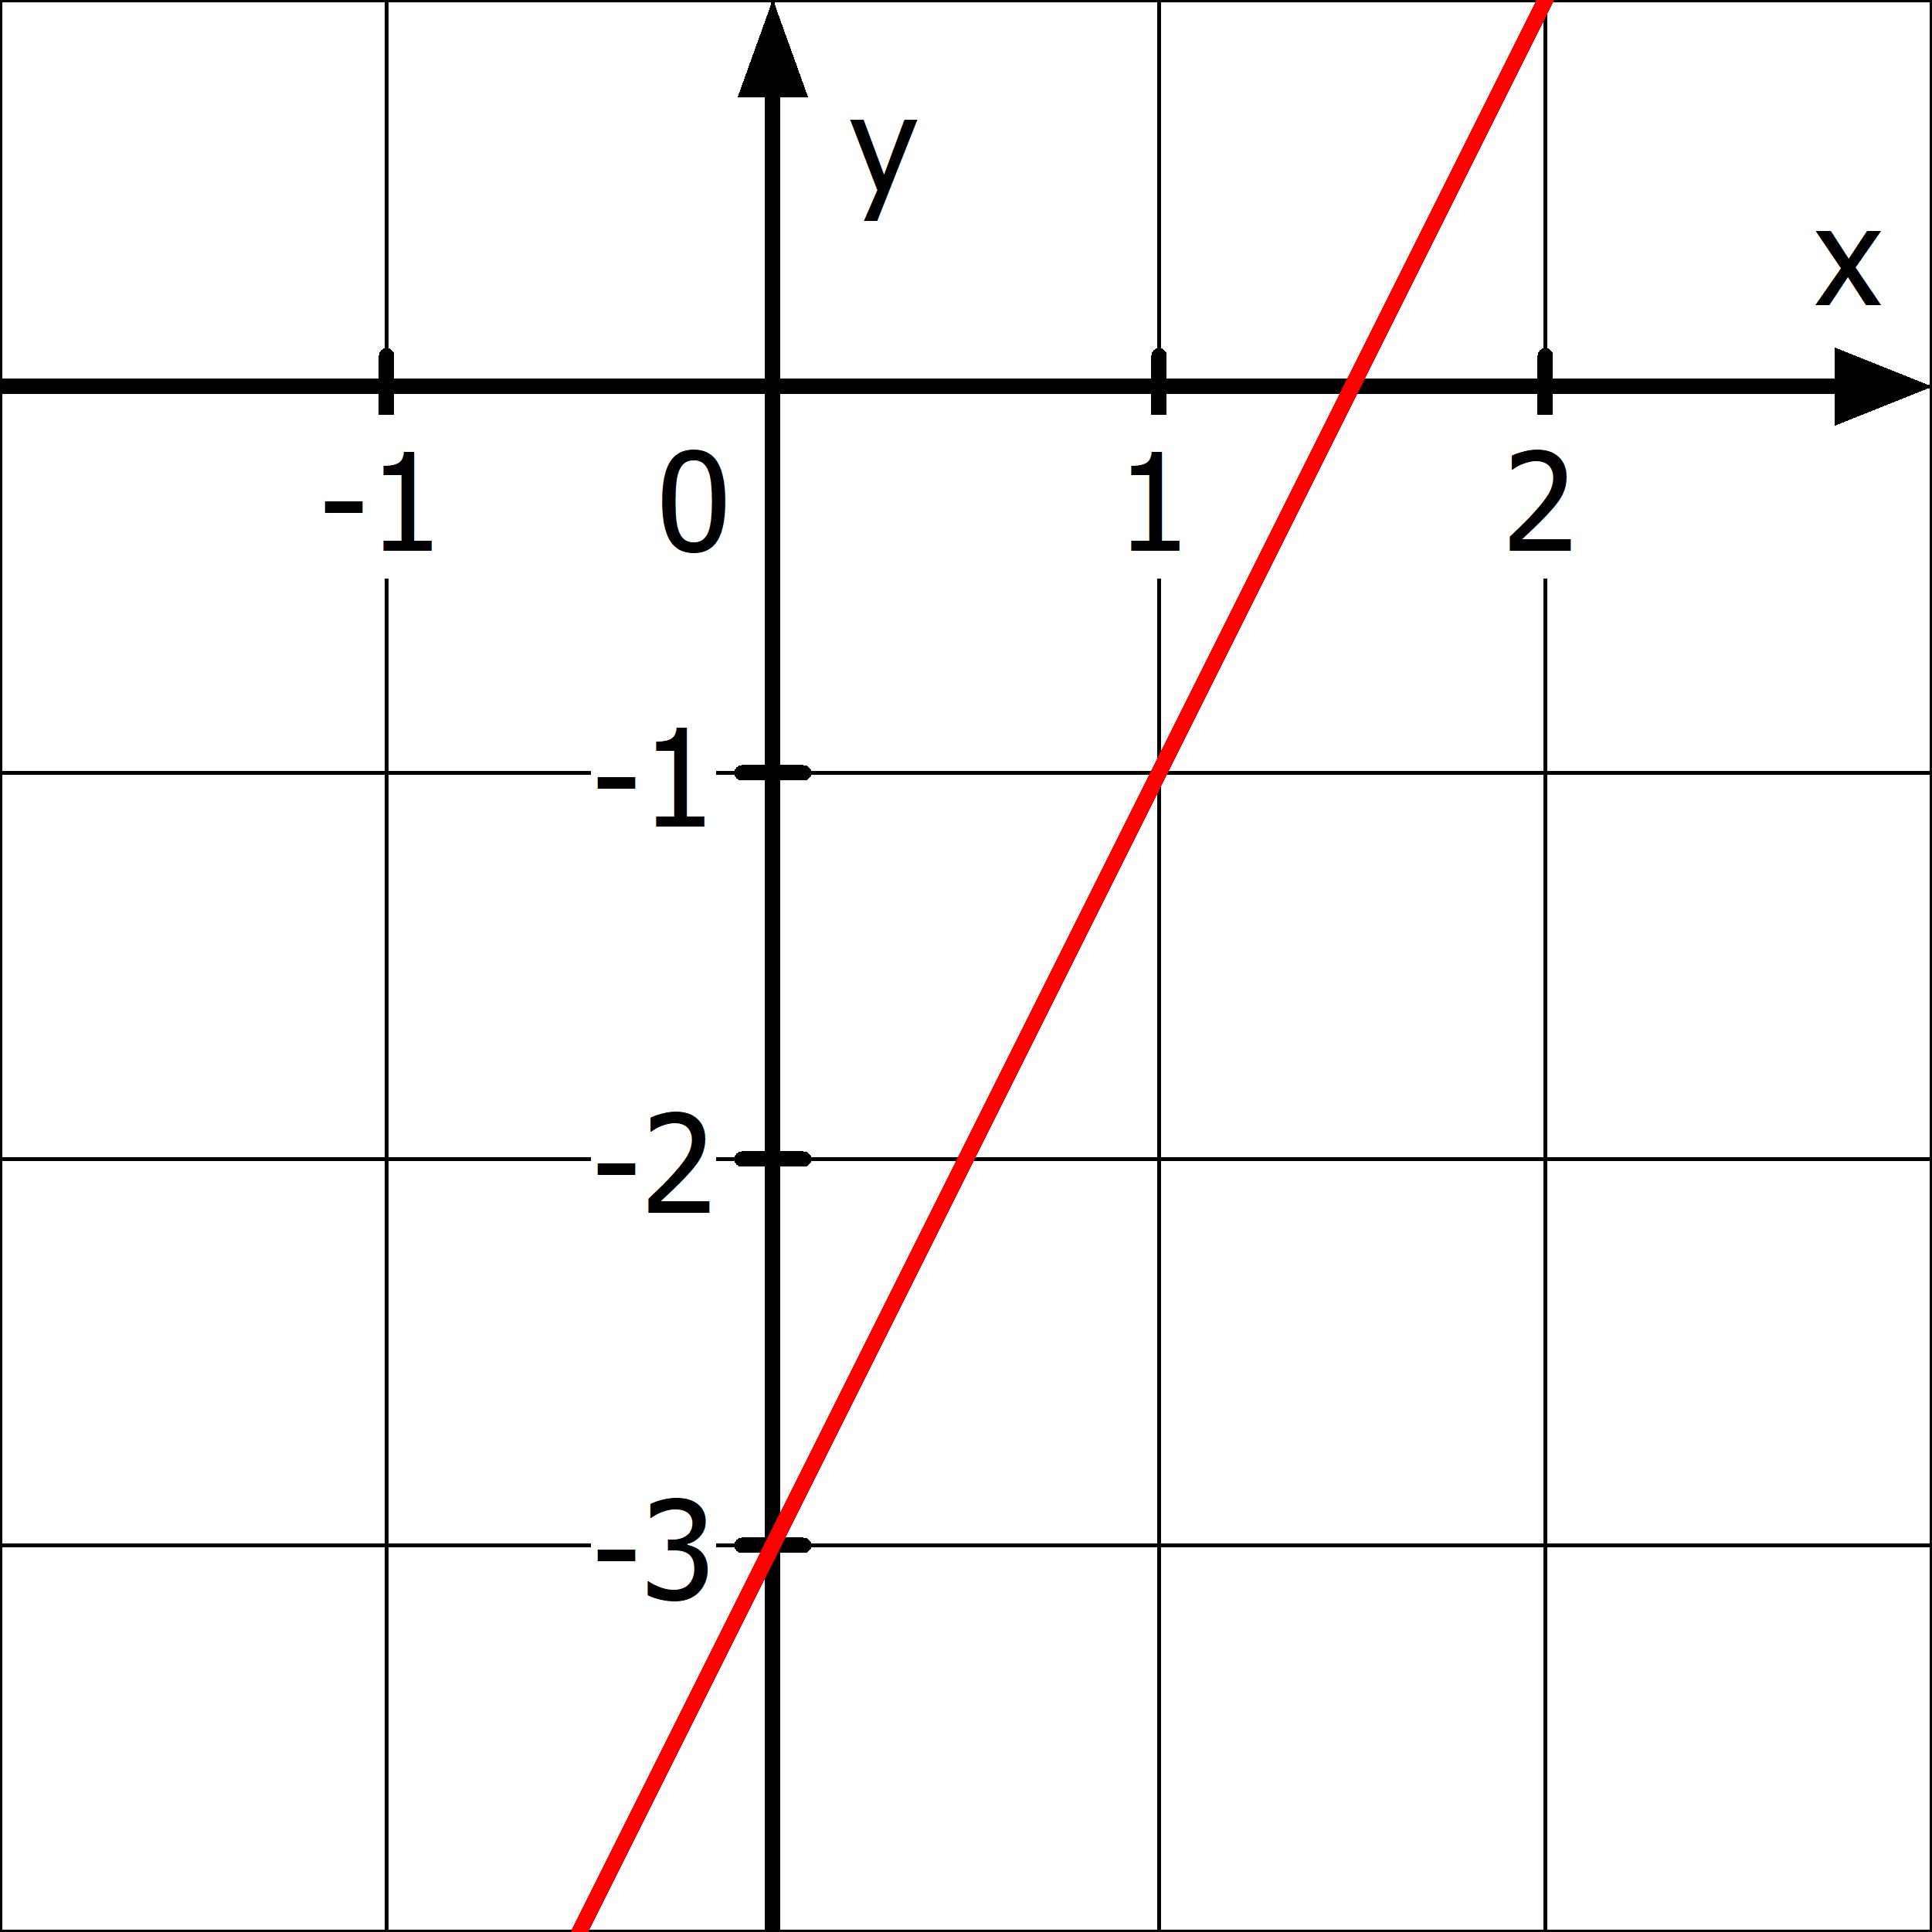
\includegraphics[width=0.4\textwidth]{\linFkt/pics/einfuehrungA1_Loesung.png}&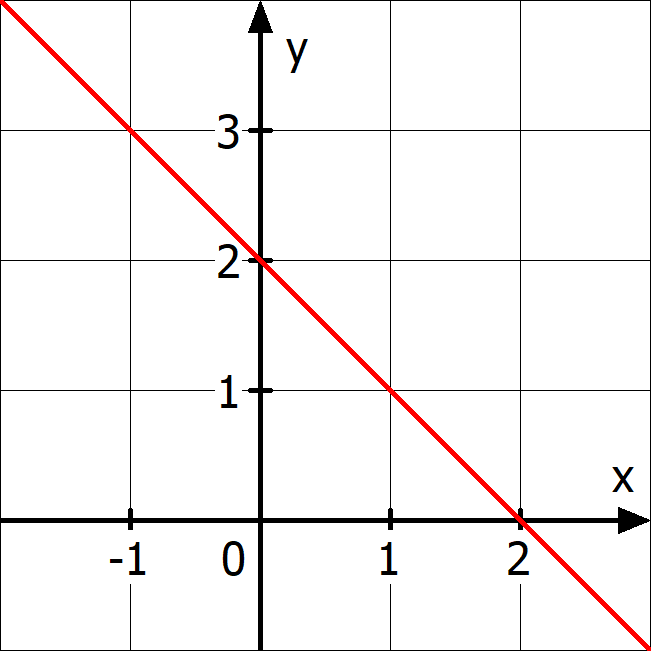
\includegraphics[width=0.4\textwidth]{\linFkt/pics/einfuehrungA2_Loesung.png}  \\
			\(f_1(x)=2x-3\)&	\(f_2(x)=-x+2\)  \\ \addlinespace[20pt]
			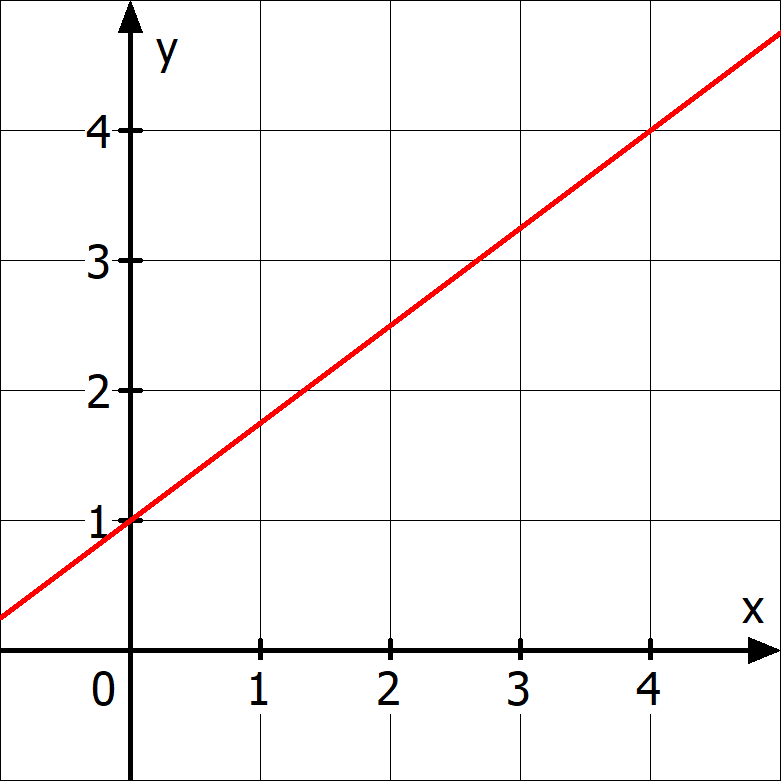
\includegraphics[width=0.4\textwidth]{\linFkt/pics/einfuehrungA3_Loesung.png}&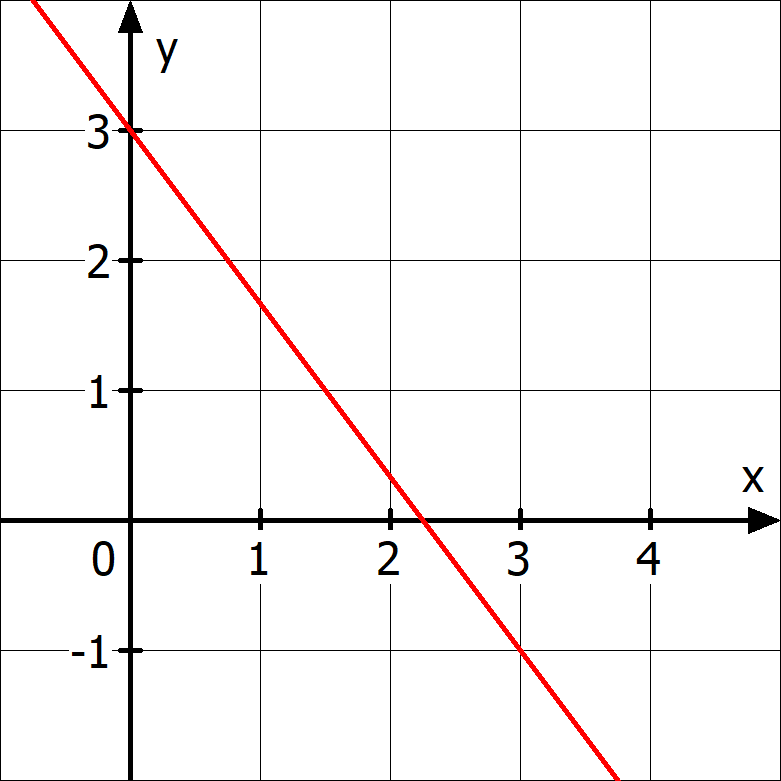
\includegraphics[width=0.4\textwidth]{\linFkt/pics/einfuehrungA4_Loesung.png}  \\
			\(f_3(x)=\frac{3}{4}x+1\)&	\(f_4(x)=-\frac{4}{3}x+3\)  \\
		\end{tabular}
	\end{minipage}
\end{Answer}
\begin{Answer}[ref=lineareFktEinfuehrungA2]

	\(f_5(x)=-3x\qquad f_6(x)=-\frac{1}{3}x+1\qquad f_7(x)=\frac{3}{2}x-2\qquad f_8(x)=\frac{7}{5}x+2\)
\end{Answer}